%----------------------------------------------------------------------------
\chapter{Elméleti megalapozás} \label{chapter5}
%----------------------------------------------------------------------------
A \cite{9} cikket tanulmányozva láthatjuk, hogy az elmúlt években a biometrikus azonosítási technikák tűntek legígéretesebb lehetőségként az egyének felismerésére. Ezek a technikák az egyén fizikai és viselkedési jellemzőit vizsgálják, hogy azonosítsák és megállapítsák személyazonosságát, ahelyett, hogy jelszavak, PIN-kódok, intelligens kártyák, plasztikkártyák, tokenek vagy kulcsok segítségével hitelesítenék az embereket. A jelszavakat és a PIN-kódokat nehéz megjegyezni, és kitalálhatók; a kártyák, kulcsok és hasonlók könnyen elveszíthetők, ellophatók vagy sokszorosíthatók; A mágneskártyák megsérülhetnek és olvashatatlanná válhatnak. Az egyén biológiai tulajdonságait azonban nem lehet elfelejteni, ellopni vagy hamisítani. \cite{10}
Az arcfelismerés az egyik legkevésbé tolakodó és leggyorsabb módszer, összehasonlítva más technikákkal, például az ujjlenyomat- és íriszfelismeréssel.
Az arcfelismerés számos alkalmazásban való felhasználásának köszönhetően jelentős figyelmet kapott mind a kutatói közösségek, mind a piac részéről, és egyre nagyobb igény mutatkozott olyan robusztus arcfelismerő algoritmusok iránt, amelyek képesek kezelni a valós arcképeket.

Az arcfelismerő rendszerek általában két mechanizmus valamelyike szerint működnek: 

\begin{itemize}
    \item Ellenőrzés (egy az egyhez): két arckép közötti hasonlóságot mérik.
    \item Azonosítás (egy a sokhoz): egy adott arckép és egy nagy adatbázisban lévő összes arckép közötti hasonlóság kiszámításra kerül.
\end{itemize}

Az arcfelismerés magában foglalhatja az arcél-észlelést, a szegmentálást és a lokalizációt.
Az észlelt arcképek közvetlen arcfelismerésre való használata bizonyos hátrányokkal jár. Először is, minden javítás általában több mint 1000 pixelt tartalmaz, ami túl nagy ahhoz, hogy robusztus felismerő rendszert tudjanak létrehozni. Másodszor, az arcképek különböző kameraállásokból készülhetnek, eltérő arckifejezésekkel, megvilágítással. Ezen hátrányok kiküszöbölése érdekében különböző műveleteket hajtanak végre a detektált képeken, ilyen például a méretcsökkentés, zajtisztítás, stb.
\newpage
Az általános arcfelismerő rendszer fő összetevőit a ~\ref{fig:face1} ábra szemlélteti.

\begin{figure}
	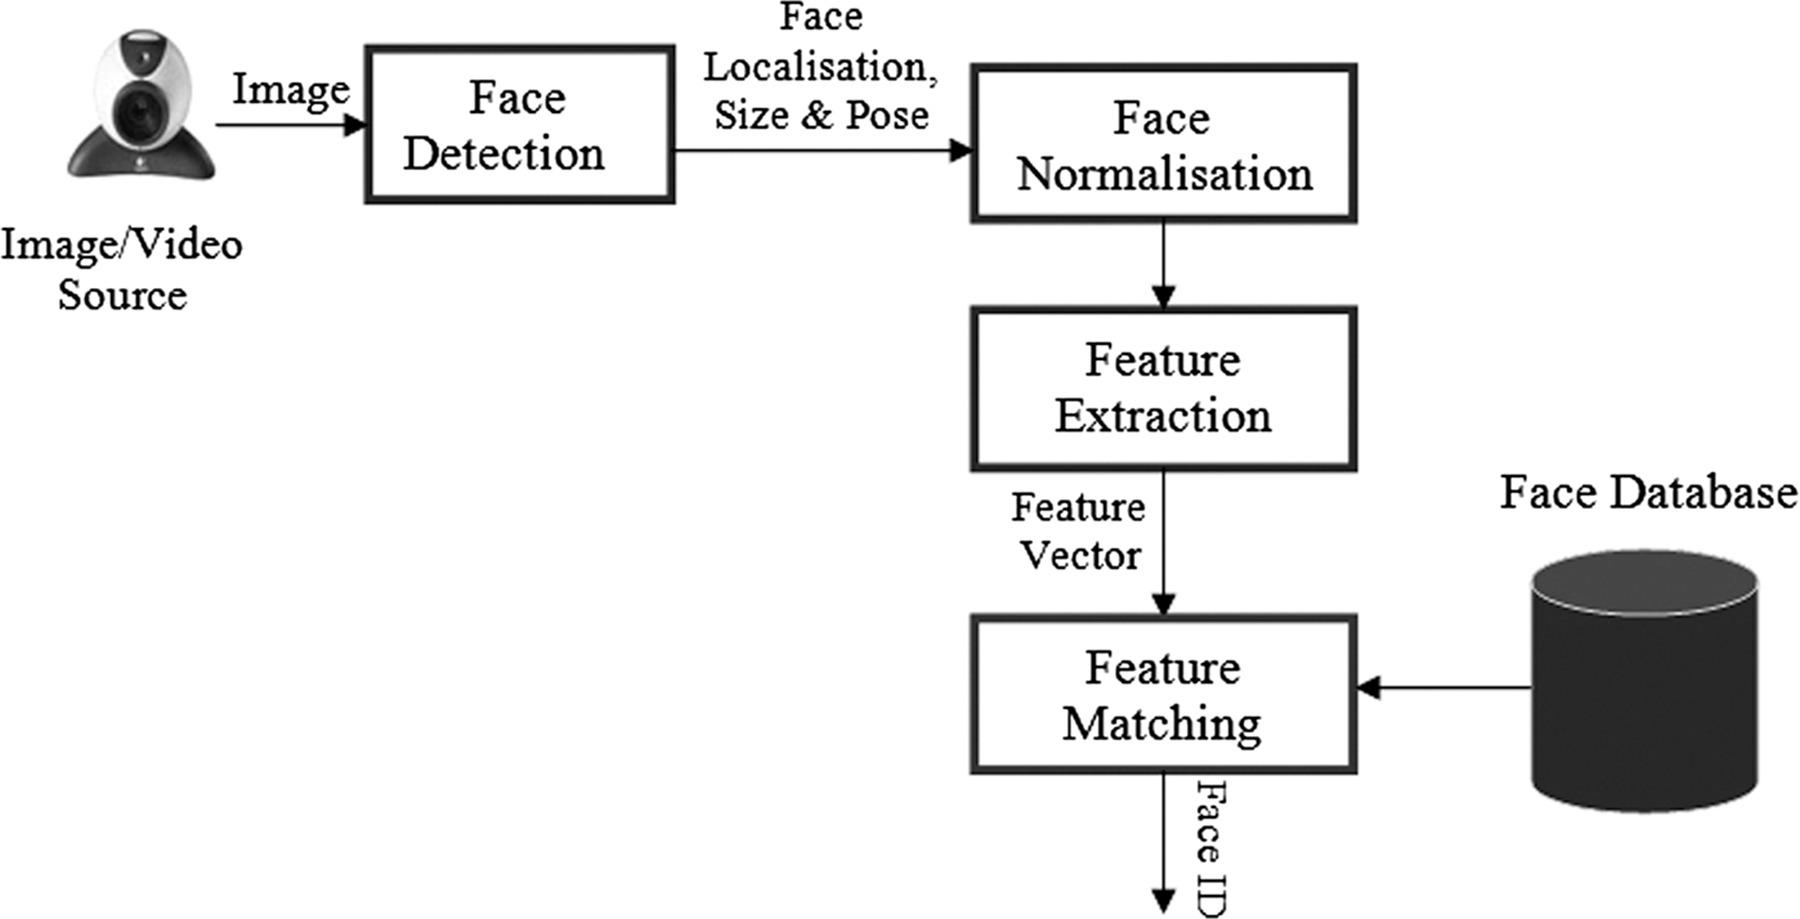
\includegraphics[width=\textwidth]{figures/facedetection_components.jpeg}
	\caption{Egy általános arcfelismerő rendszer blokkdiagramja \cite{9}}
	\label{fig:face1}
\end{figure}

\section{Az arcfelismeréssel kapcsolatos kihívások}
Általánosságban elmondható, hogy a digitális képalkotásban a jól működő arcfelismerésnek számos hátráltató tényezője ismert: váltakozó fényviszonyok, a nagy pózváltozatok, a különböző arckifejezések, a smink, az arcszőrzet változásai, az öregedés.
Valójában számos kihívás és kulcstényező van, amelyek jelentősen befolyásolhatják az arcfelismerési teljesítményt. Ezen kihívások közül néhányat a ~\ref{fig:face2} ábra szemléltet, amelyek az alábbi kategóriákba sorolhatók:

\begin{enumerate}[label=(\alph*)]
    \item Kihívások a fényviszonyok változásai miatt
    \item Kihívások a pózváltozás miatt
    \item Kihívások az öregedési változások miatt
    \item Kihívások az arckifejezés/arcstílus miatt
    \item Kihívások az eltakarás miatt
\end{enumerate}

\begin{figure}
	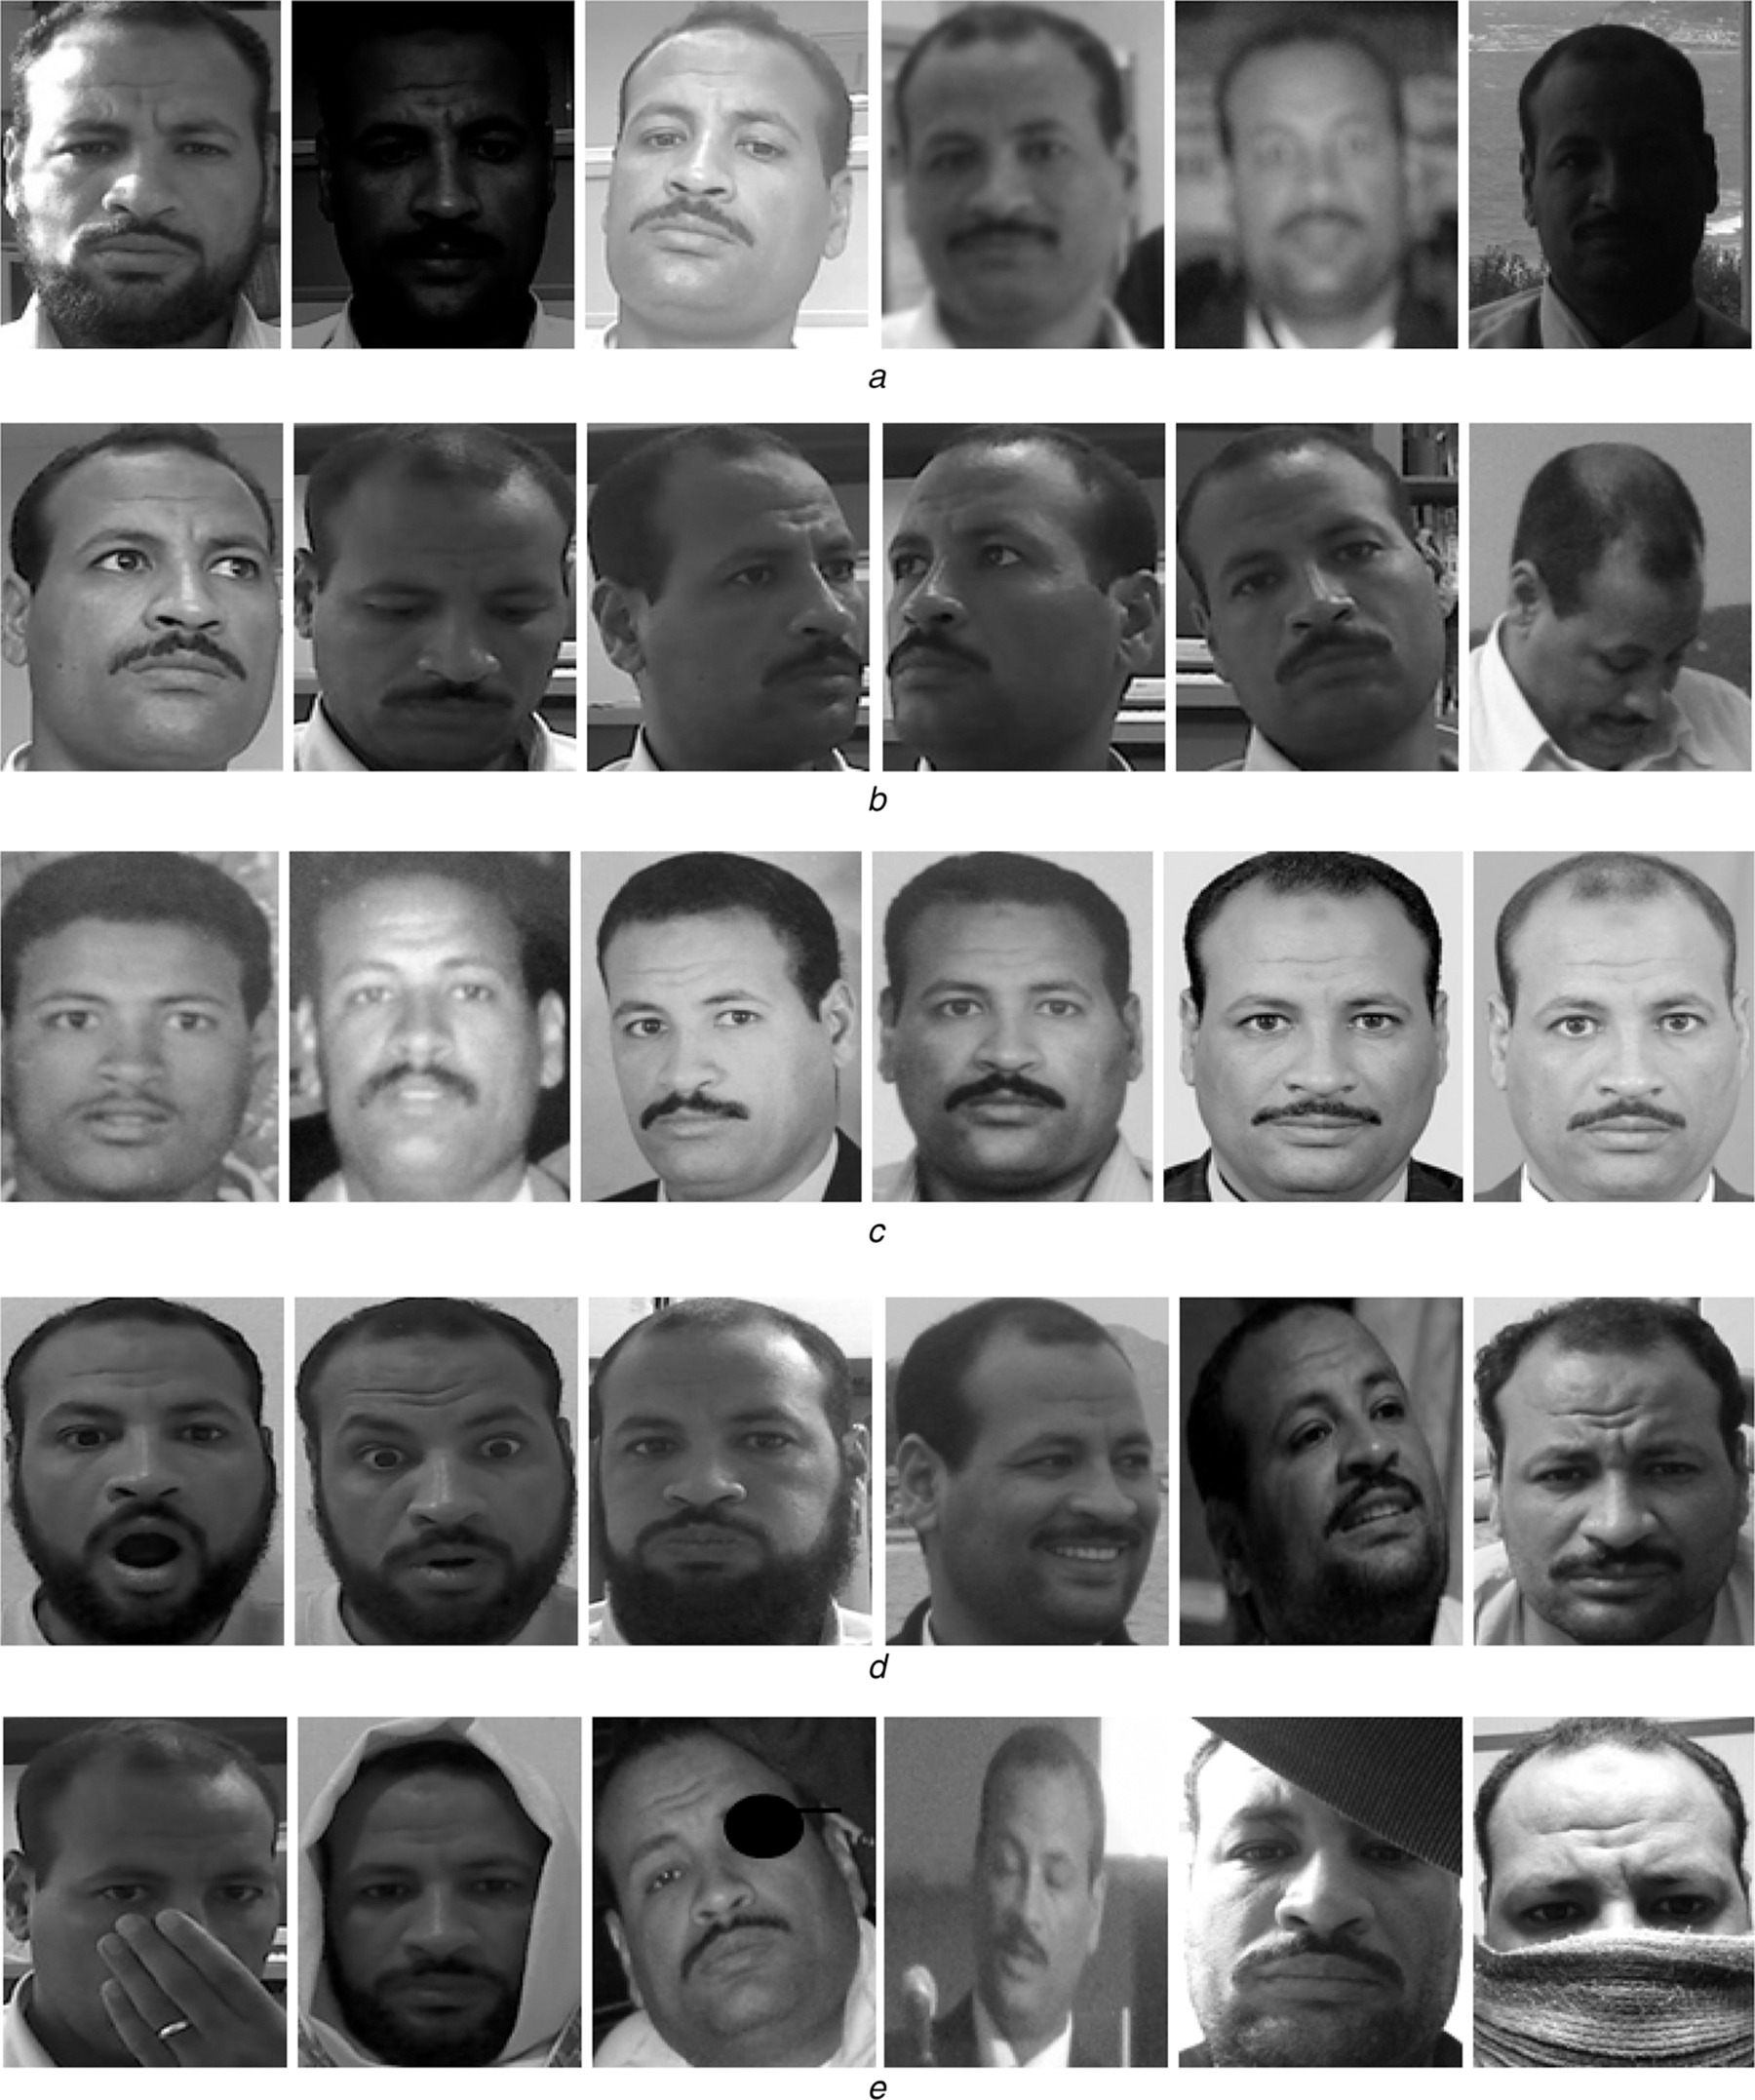
\includegraphics[width=\textwidth]{figures/facedetection_challenge.jpeg}
	\caption{Arcfelismerést nehezítő kihívások szemléltetése \cite{9}}
	\label{fig:face2}
\end{figure}

\newpage

\subsection{Megvilágítási variációk}
A kép kialakítása során olyan tényezők, mint a megvilágítás (spektrumok, forráseloszlás és intenzitás) és a kamera jellemzői (érzékelő reakciója és lencsék) bizonyos mértékig befolyásolják az emberi arc megjelenését.
Egy robusztus és hatékony arcfelismerő rendszer kivitelezése során a megvilágítás problémáját tekintik a rendszertervezők előtt álló egyik fő műszaki kihívásnak, ahol az ember arca eltérőnek tűnhet a fényviszonyok tekintetében \cite{11}.
A megvilágítás variációira vonatkozó jelenlegi megközelítések többsége erős feltételezéseket tesz, amelyeket a gyakorlatban nagyon nehéz teljesíteni.
A fényviszonyok vagy a pózok változásainak kezelésére a póz-robusztus albedóbecslésen alapuló képújravilágítási technika használható ugyanazon személy több frontális képének előállítására változó megvilágítás mellett \cite{12}. Az albedóbecslés egyik korlátja az, hogy a képek egymáshoz igazítását, valamint az arckifejezésekre való érzékenységet igénylik.


\subsection{Póz/nézőpont}

Az arcképek a kamera viszonylagos arcpózától függően változnak (elülső, 45°-os, profil, fejjel lefelé), és egyes arcvonások, például a szemek vagy az orr részben vagy teljesen eltakaródhat. Valójában a pózváltozások hatással vannak a felismerési folyamatra. Így a póztolerancia még kritikusabbá válik azoknál az arcfelismerő rendszereknél, amelyek az alany egyetlen nézetén alapulnak \cite{13}.


Blanz és munkatársai \cite{14} a nézőpontos arcfelismerési módszereket két alternatív paradigmába sorolta:  

\begin{itemize}
    \item Nézőpont-transzformált: előfeldolgozási módon működnek, és a becsült pózparaméterek alapján átalakítják a próbaképet, hogy azok illeszkedjen a galériában lévő képhez.
    \item Együttható alapú: megkísérli egyetlen kép alapján megbecsülni az arc fényterét; ez megtörténik a galéria és a próbaképek esetében is.
\end{itemize}

A póz problémájának megoldását 2D és 3D adatok kombinációjával is vizsgálják.


\subsection{Öregedés és ráncok}

Az öregedés lehet természetes (az életkor előrehaladása miatt) és mesterséges (sminkeszközök használata).
Az öregedés és a ráncok mindkét esetben súlyosan befolyásolhatják az arcfelismerő rendszerek teljesítményét. Általánosságban elmondható, hogy az arcfelismerési kutatások során általában nem veszik figyelembe az életkor változásának hatását. Az egyik fő oka annak, hogy az arcfelismeréssel kapcsolatos, életkori tényezővel összefüggésben megvalósuló tanulmányok kis száma miatt nem állnak rendelkezésre reprezentatív nyilvános adatbázisok, amelyek különböző életkorú egyéneket tartalmazó képeket tartalmaznának, valamint közrejátszik a régi képek alacsony minősége is, amint azt a szakirodalom dokumentálja.\cite{15}. Nagyon nehéz olyan arcképekhez olyan adathalmazt gyűjteni, amely ugyanarról a személyről, élete során, különböző életkorban készült képeket tartalmazna.


\subsection{Arckifejezés/arcstílus}

Az arcok megjelenését közvetlenül befolyásolja a személy arckifejezés. Az arcszőrzet, például a szakáll és a bajusz megváltoztathatja az arc megjelenését és az arc alsó felében, különösen a száj és az áll környékén. Ezenkívül a frizura megváltoztatható az arckép megjelenésének megváltoztatása vagy az arcvonások elrejtése érdekében. Aleix \cite{16} úgy fogalmazza meg az arcfelismerés problémáját az arckifejezés alatt, hogy „hogyan lehet robusztusan azonosítani egy olyan személy arcát, akinél a tanuló és a tesztelő arcképek arckifejezésében különböznek?”


\subsection{Eltakarás}

Az arcokat más tárgyak részben eltakarhatják. Egy embercsoportot ábrázoló képen egyes arcok vagy más tárgyak részben elfedhetnek más arcokat, ami viszont azt eredményezi, hogy sok helyzetben az arcnak csak egy kis része lesz látható. Ez azonban nehéz feladattá teszi az arcfelismerést a rendszer helye alapján, és még ha az arcot megtalálják is, maga a felismerés nehézségekbe ütközhet az arc egyes rejtett részei miatt, ami megnehezíti a felismerést \cite{17}.


\section{A személyazonosság-hitelesítési módszer, amely ötvözi az életszerűség-érzékelést (liveness) és az arcfelismerést}

A nagy sebességű processzorok és a nagy felbontású kamerák megjelenése a kutatás élére állt az arcfelismerő rendszerek különféle alkalmazásokhoz történő tervezésére. Az arcfelismerő rendszerek az alkalmazástól függően offline adatokat vagy valós idejű bevitelt használnak.


A \cite{18} tanulmányban egy fejlett Kinect érzékelőt alkalmaztak az életszerűség észleléséhez. Az infravörös sugárzás (IR) felvételeken alapuló életszerűség-észlelési módszer képes kezelni az archamisításokat. A jellemzők kinyerését és osztályozását egy mély neurális háló hajtotta végre, hogy különbséget tegyen a valódi személyek és az archamisítások között. A Kinect kamera által gyűjtött infravörös képek mélységi információkat tartalmaznak. Ezért az élő képek infravörös képpontjainak nyilvánvaló hierarchikus szerkezete van, míg a fényképek vagy videók képpontjainak nincs nyilvánvaló hierarchikus jellemzője. Ennek megfelelően kétféle IR-képet tanultak meg a mélyhálón keresztül annak megállapítására, hogy a képek élő egyedektől származnak-e. Más életszerűség-detektáló keresztadatbázisokkal összehasonlítva felismerési pontosságunk 99,8 százalék volt, és jobb, mint más algoritmusok. A FaceNet egy arcfelismerő modell, amely robusztus az elmosódáshoz és a megvilágításhoz. A személyazonosság-hitelesítéshez kombinálták az életszerűség-érzékelést és a FaceNet modellt. A kísérleti eredmények azt mutatták, hogy a javasolt életszerűség-érzékelés és a továbbfejlesztett arcfelismerés kombinációja jó felismerő hatással bír, és felhasználható személyazonosság-azonosításra.

Az arcfelismerés pontossága nagymértékben javul a mély tanulási hálók használatával, mivel képes kiemelni az emberi arcok mély vonásait.

Bár a továbbfejlesztett FaceNet keretrendszer más felismerő rendszerekhez hasonlóan pontosan képes felismerni az emberi arcokat, nem tudja megakadályozni a csalást. A legtöbb létező arcfelismerő rendszer sebezhető a hamisító támadásokkal szemben. Hamisító támadásról akkor beszélünk, ha valaki megkísérli megkerülni az arc biometrikus rendszerét, hamis arcot mutatva a kamera előtt.

A \cite{18} cikk olyan életszerűség-érzékelési megközelítést javasol, amely a Kinect kamerával nyert infravörös sugárzás (IR) képeken alapul. Az élő arcok infravörös képei pozitív mintaként jelennek meg, míg a fényképek vagy videók infravörös képei negatív mintaként. A fenti minták bemenetre kerülnek a konvolúciós neurális hálóba (CNN), hogy megtanulják az élő arcokat és a hamis támadásokat. Az életszerűség észlelése után a továbbfejlesztett FaceNet továbbra is felismeri az arcokat, és biztosítja a megfelelő azonosítót vagy az UNKNOWN kimenetet a pontos azonosítás érdekében.

Az arcfelismerés fokozatosan fontos titkosítási és visszafejtési módszerré vált gyorsasága, hatékonysága és felhasználóbarát jellege miatt. Az arcfelismerő technológia biztonsági kérdései azonban egyre hangsúlyosabbak. Ezért az életszerűség-érzékelés a megbízható hitelesítési rendszerek fontos részévé vált.

A gyakori hamisított arcok közé tartoznak a fényképek (nyomtatott), a videók (visszajátszás), a maszkok és a szintetikus 3D arcmodellek. Köztük a fotók és videók 2D hamis arcok, amelyek olcsóbbak a hamis támadásokhoz, és a megtévesztés két legnépszerűbb formája. Ezért az arcfelismerés gyakorlatiasságának és biztonságának javítása érdekében be kell vezetni az életszerűség-érzékelést a személyazonosság-hitelesítési rendszerekbe. 

Az elterjedt életszerűség-érzékelési módszerek főként textúrán, életinformációkon, különböző érzékelőkön és mély jellemzőkön alapulnak. Az élő arcok összetett 3D-s szerkezetekkel rendelkeznek, míg a fotó- és videótámadások 2D-s síkstruktúrák. A 3D és 2D struktúrák felületeinek különböző fényvisszaverődései különbségeket mutatnak az arcszínek világos és sötét területein. A textúra alapú módszerek főként ezeket a különbségeket használják támpontként az élő és a hamis arcok osztályozására. A textúrán alapuló detektálási módszert Local Binary Pattern (LBP) \cite{19} és továbbfejlesztett LBP \cite{20} algoritmusok segítségével valósítják meg. Ez a módszer alacsony számítási bonyolultságú és könnyen megvalósítható, de a hardverkörülmények nagymértékben befolyásolják. Az algoritmus pontossága csökken, ha a képminőség alacsony.

Az életjellemzőkre épülő módszer olyan életjeleket használ, mint a szívverés, a véráramlás, a pislogás és az arcizmok akaratlan mikromozgása az élő és a hamis arcok osztályozására. A kényszerfeltételek mellett ez a módszer nagy észlelési pontossággal rendelkezik, ha az életjellemzők stabilan kinyerhetők; ez a módszer azonban arcvideót igényel bemenetként, és nagy mennyiségű számítást igényel.

A különböző szenzorokon alapuló módszer különböző képgyűjtő rendszereket alkalmaz, például multispektrális kamerát, infravörös kamerát, mélykamerát, hogy megfelelő típusú emberi arcképeket rögzítsen az életszerűség érzékeléséhez. Ennek a módszernek az általános felismerési pontossága magas, de ehhez a módszerhez új hardvert kell hozzáadni, és így megnő a rendszer költsége. A mély jellemzőkre épülő módszerek magukban foglalják a kezdeti CNN tanítását a mélységi jellemzők kinyerésére, majd az osztályozást. Az arcfelismerő rendszerek fokozatos elterjedésével és a hardverek drágulásával szükséges és érdemes néhány fontos architelesítési rendszerbe képrögzítő berendezéseket beépíteni, azok biztonságának és megbízhatóságának javítása érdekében. Az arcok életszerűség-érzékelését valós mélységinformáció segítségével nem használják általánosan a biometrikus technológiában és a szakirodalomban.


\subsection{Módszertan}

Az infravörös képeket egy Kinect kamera rögzítette tanulóadatokként. A valódi arcokról származó adatok pozitív mintaként, míg a fotók vagy videók negatív mintaként szolgáltak arra, hogy a CNN-hálót megtanítsák annak megállapítására, hogy egy arc élő-e. Ezen túlmenően, mivel a FaceNet modell nagy arcfelismerési pontossággal rendelkezik, a továbbfejlesztett FaceNet élénkség-érzékelő algoritmussal kombinálva integrált hitelesítési rendszert alkot.

Az ~\ref{fig:face3} ábrán látható a javasolt keretrendszer, amely a FaceNet-et az élénkségérzékeléssel kombinálja, ahol CNN, konvolúciós neurális háló;  IR, infravörös sugárzás; MTCNN, többfeladatos kaszkádos CNN.


\begin{figure}[htbp]
	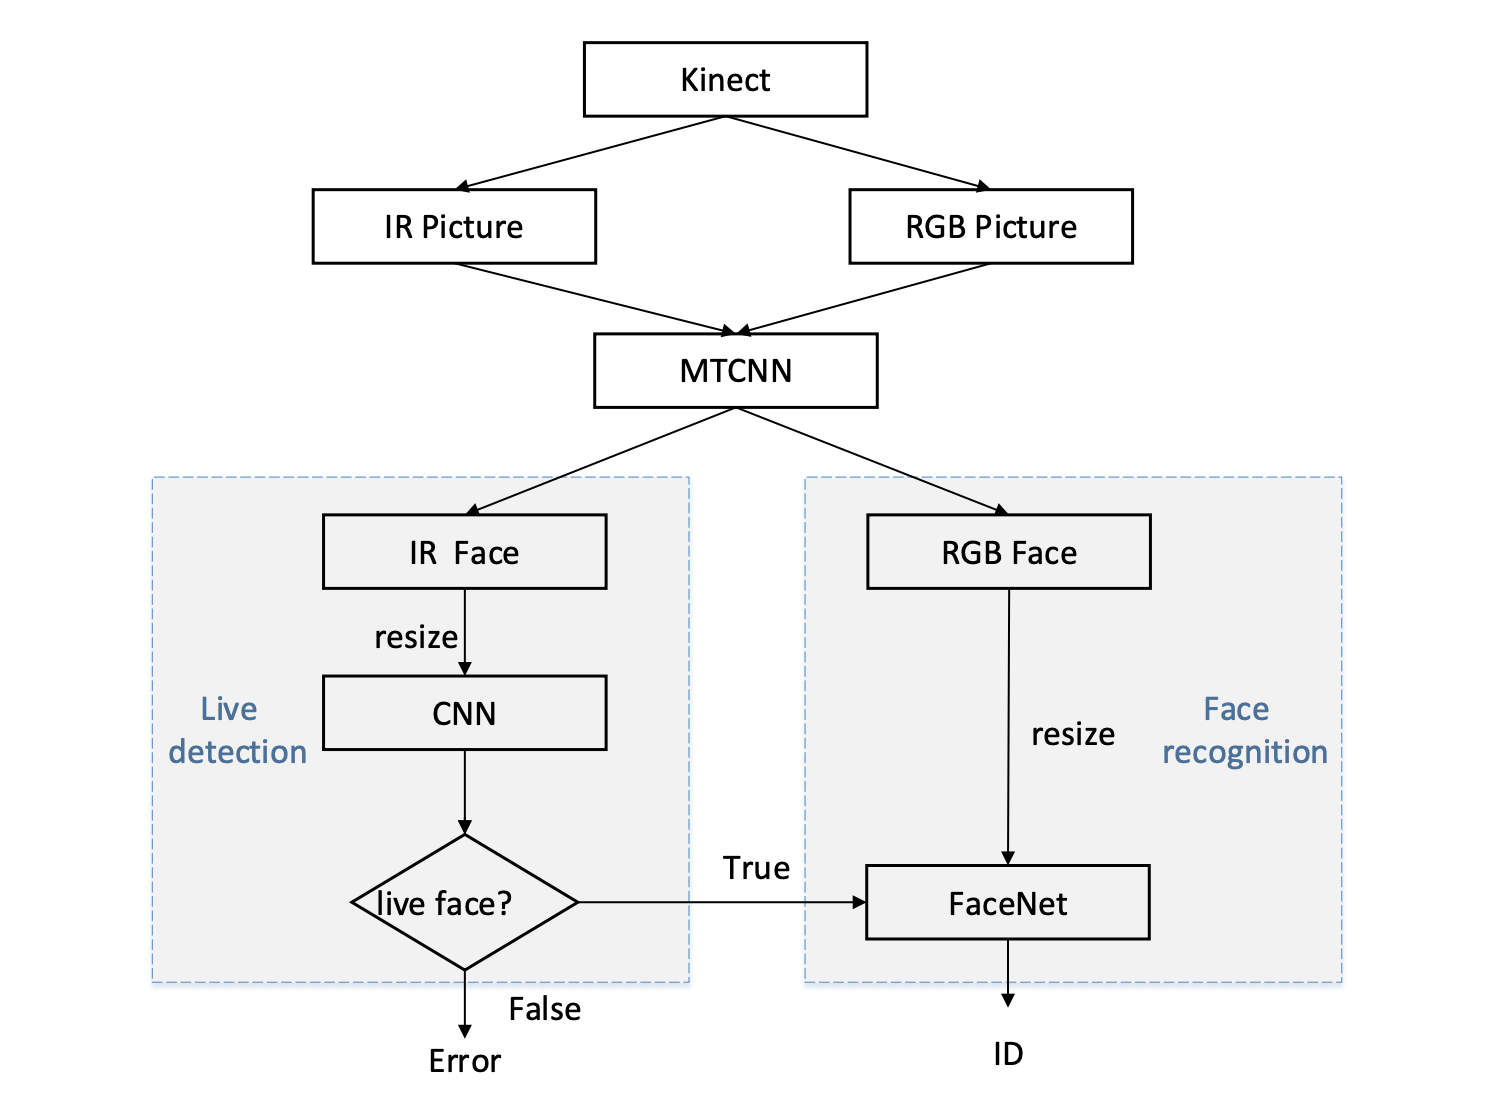
\includegraphics[width=\textwidth]{figures/live_rec.png}
	\caption{Életszerűség-érzékelésen és FaceNeten alapuló identitás-hitelesítési keretrendszer \cite{18}}
	\label{fig:face3}
\end{figure}

Először egy Microsoft Kinect kamerát használtak, amellyel RGB és IR képeket gyűjtöttek az emberi arcokról. Másodszor, egy multitask kaszkád konvolúciós hálót (MTCNN) használtak az RGB és IR képek arcrészeinek vágására és igazítására. Végül az MTCNN által feldolgozott infravörös képeket a CNN életszerűség-érzékelésére, míg az RGB képeket a FaceNet modell arcfelismerésre való betanítására használták. Ha az életszerűség-érzékelés eredményei igazak, az arcfelismerés folytatódik a teljes hitelesítési folyamat befejezéséhez. Ha az életszerűség-érzékelés hamis, akkor az algoritmus működése leáll, és az arcfelismerés többé nem történik meg.

\subsection{Életszerűség-érzékelés IR képjellemzők alapján}

Az IR képeken alapuló archamisítás-felismerés kétosztályos problémaként kezelhető. Ez a módszer a hamis arcok és a valódi arcok megkülönböztetésére szolgál. A javasolt életszerűség-érzékelési algoritmus a 3D arctér becslésére összpontosított. Kinect kamerát használtak a mély és szürke információkat tartalmazó infravörös képek készítéséhez. Ezeket a képeket bevitték a CNN-be, hogy megtanítsák az arcbőr textúrájára vonatkozó információkat. Mivel a teljes arctextúrákat figyelembe vették, a 2D-s megtévesztéseknek, például a fényképeket és videókat használóknak, már nincs hatása. Pozitív mintaként valós arcokról és bekeretezett valós arcokról készült IR-felvételek, negatív mintaként fotók, emberi arcokra ragasztott fotók és elektronikus eszközökön lévő fotók készültek, amiket aztán a CNN kapott meg, ahogy azt a ~\ref{fig:face3} ábra szemlélteti.

\begin{figure}[htbp]
	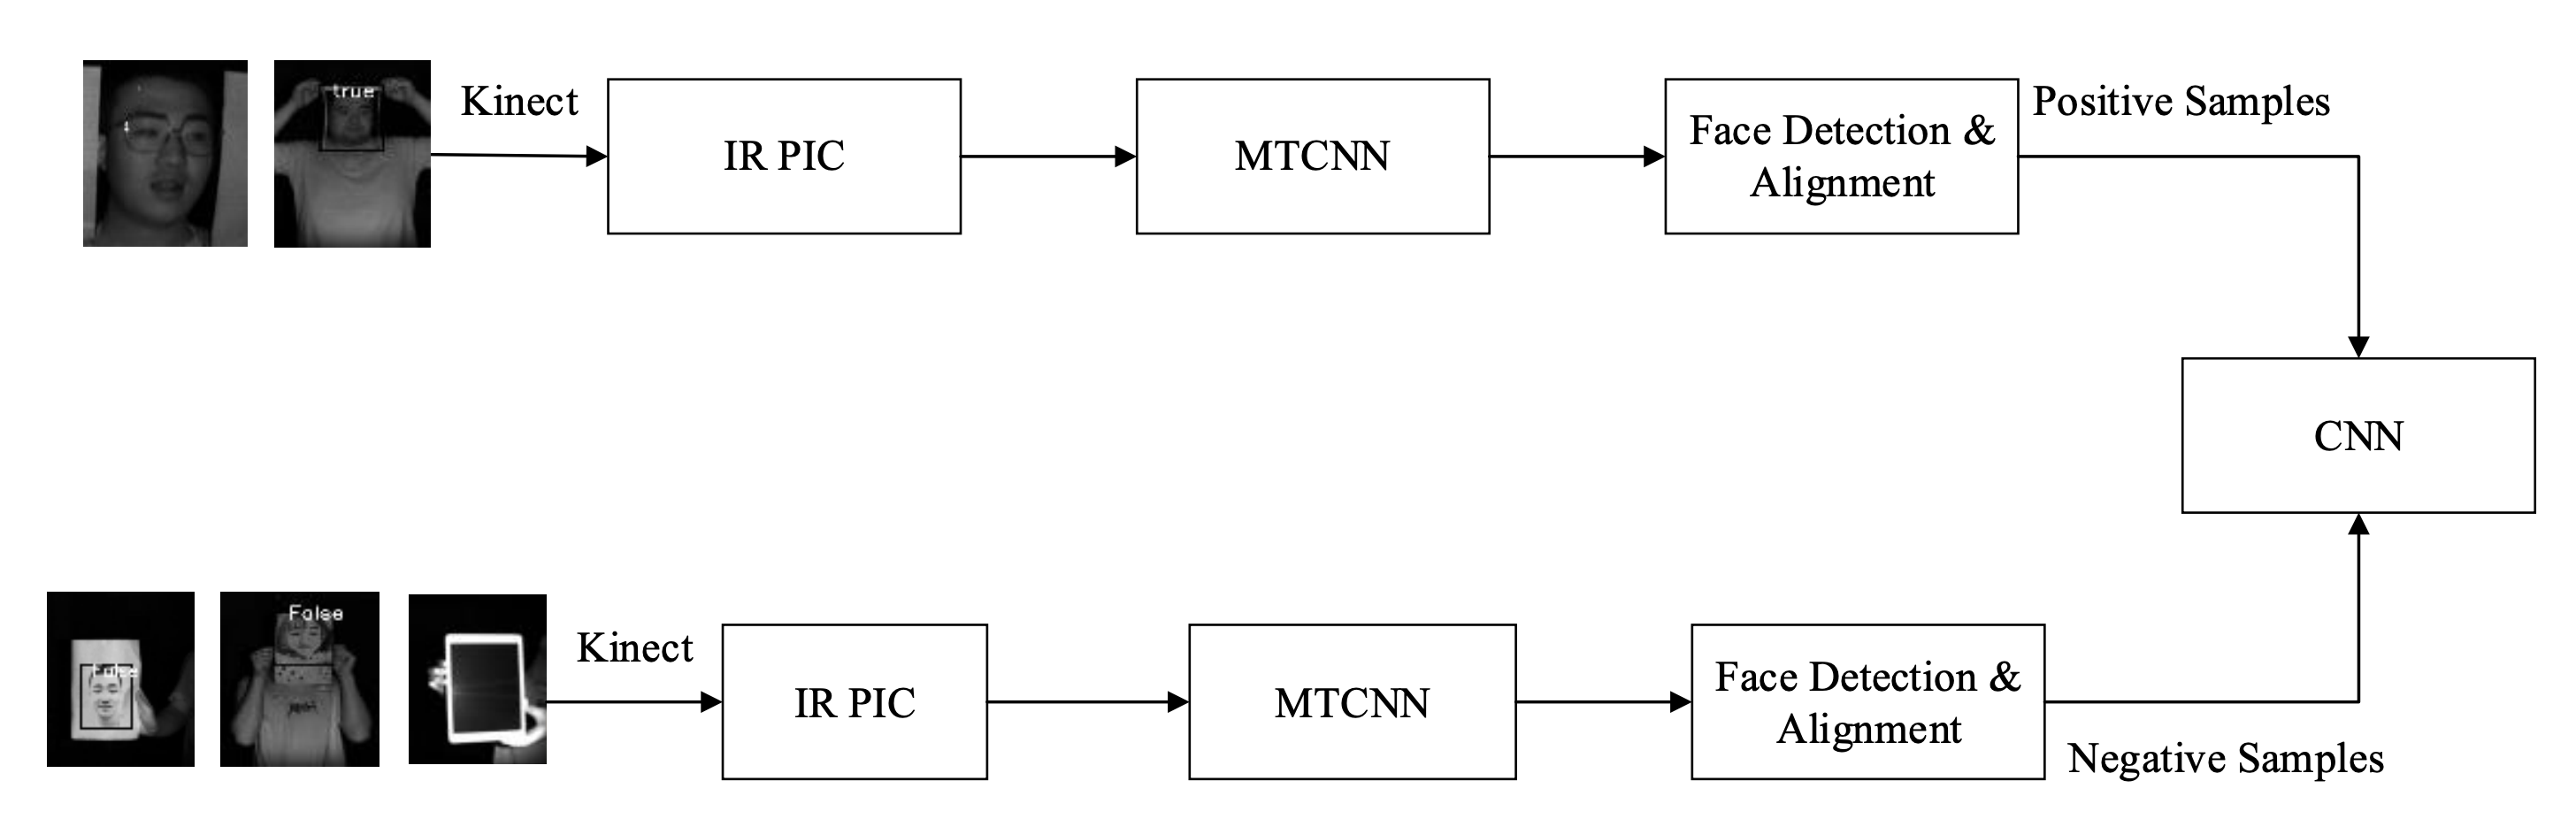
\includegraphics[width=\textwidth]{figures/live_training.png}
	\caption{Életszerűség-érzékelés tanulási folyamata \cite{18}}
	\label{fig:face4}
\end{figure}

\subsection{Összegzés}

Az olvasott tanulmány egy személyazonosság-hitelesítési rendszert javasolt, amely egy továbbfejlesztett FaceNet-modellt és egy életszerűség-észlelési módszert kombinál. A Kinect kamera által gyűjtött infravörös képek mélységi információkat tartalmaznak. Ezért az élő képek infravörös képpontjainak nyilvánvaló hierarchikus felépítése van, míg a fényképek vagy videók képpontjai nem rendelkeznek ezzel a funkcióval. A rendszer hatékonyan képes észlelni a 2D megtévesztést. Az élő arcok infravörös képi jellemzői nagymértékben eltérnek a fényképek vagy videókétól, így az életszerűség-észlelés bináris osztályozási problémaként kezelhető. Így a CNN-t úgy tervezték, hogy pontos életszerűség-felismerést valósítson meg. Az algoritmus nagy időhatékonyságú volt, és valós időben is alkalmazható.

\newpage

\section{Arcfelismerő modellek: melyiket használjuk és miért?}

A következőkben a \cite{21} cikk alapján olyan előre betanított modelleket vizsgálunk, mint a Haar-kaszkádok, a dlib frontális arcdetektor, az MTCNN (Multi-task Cascaded Convolutional Neural Network) és az OpenCV DNN-modulját használó Caffe modell, hogy megtudjuk, melyik működik a legjobban a valós idejű alkalmazások esetén, ezáltal melyiket érdemes használnunk a projekt kivitelezése során.

\subsection{Haar-kaszkádok (Haar Cascades)}

Gyors a munkavégzés, és az egyszerű CNN-hez hasonlóan sok jellemző kinyerésére képes a képekből. A legjobb jellemzőket ezután az Adaboost segítségével választja ki. Ez az eredeti 160 000+ jellemzőt 6000-re csökkenti, viszont mindezen jellemzők csúszóablakban történő alkalmazása még mindig sok időt vesz igénybe. Így bevezették az osztályozók kaszkádját, ahol a jellemzők csoportosítva vannak. Ha egy ablak meghibásodik az első szakaszban, akkor a kaszkád többi szolgáltatása nem kerül feldolgozásra. Ha megfelel, akkor a következő szolgáltatást tesztelik, és ugyanazt az eljárást megismétlik. Ha egy ablak képes átadni az összes jellemzőt, akkor az arcterületnek minősül.


A Haar-kaszkádok tanításához sok pozitív és negatív tanulókép szükséges. Szerencsére ezek a kaszkádok az OpenCV-könyvtárral és a betanított XML-fájlokkal együtt érkeznek.


\subsection{Dlib frontális arcérzékelő (Dlib Frontal Face Detector)}

A Dlib egy C++ eszközkészlet, amely gépi tanulási algoritmusokat tartalmaz valós problémák megoldására. Bár C++-ban van írva, különböző interfészeken keresztül lehetőségünk van Pythonban is használni. Ezenkívül rendelkezik a mérföldkőnek számító kulcspontérzékeléssel is.
A kulcspont-észlelés a kulcsobjektum-részek megtalálásából áll. Arcunk kulcsfontosságú részei például az orr, a szemöldökök, a szemzugok stb. A kulcspontérzékelés egyik fő alkalmazási területe az arcfelismerés.

A dlib által biztosított elülső arcdetektor az Orientált Gradiens Histogram (HOG) segítségével kinyert jellemzőket használ, amelyeket aztán egy SVM-en (Support Vector Machine) továbbítanak. A HOG jellemzőleíróban a színátmenetek irányainak eloszlását használjuk jellemzőként.


\subsection{Többfeladatos kaszkádos konvolúciós neurális hálózat (Multi-task Cascaded Convolutional Neural Network)}

Nem csak az arcot érzékeli, hanem öt kulcspontot is. Kaszkád struktúrát használ a CNN három szakaszával. Miután megvannak a jelöltek, ezeket átadják egy másik CNN-nek, amely visszautasítja a nagyszámú hamis pozitív eredményt, és elvégzi a határolókeretek kalibrálását. Az utolsó szakaszban az arc kulcspontjainak észlelését hajtják végre.


\subsection{DNN arcérzékelő az OpenCV-ben (DNN Face Detector in OpenCV)}

Ez egy Caffe modell, amely az SSD-n (Single Shot-Multibox Detector) alapul, és a ResNet-10 architektúrát használja. Az OpenCV 3.3 után került bevezetésre a mély neurális hálózati moduljában.

\subsection{A képeken elért eredmények összehasonlítása}

A tanulmány során a modellek teszteléséhez két típusú képeket használtak: nagy méretű és felbontású Unsplash fotókat és kis méretű Google fotókat.
Az első esetben mivel a képek átlagos mérete 5000x5000 körül volt, a feldolgozás előtt a magasságot és a szélességet is felére kellett csökkenteni. Míg a Google képek esetén az átlagos képméret 220x220, feldolgozásuk az eredeti állapot szerint történt, kivéve a DNN-modult, ahol a képeket 300x300-ra méretezték át, mivel az eredmény nem volt jó, ha eredeti méretű képeket használtak.

Mindezek alapján alkalmazva a négy modellt, a következő eredmények születtek:

\begin{itemize}
    \item A Haar eléggé elavult, és általában a legrosszabb eredményeket adta.
    \item Az OpenCV DNN moduljának arcfelismerő modellje jól működött, de ha a kép mérete nagyon nagy, az problémákat okozhat. Általában nem dolgozunk ilyen 3000x3000-es képekkel, így ez ebben az esetben nem számít akkora problémának.
    \item A Dlib nem érzékeli a 80x80-nál kisebb arcokat, így ha kis képekkel dolgozunk, győződjünk meg arról, hogy felskáláztuk őket, de ez megnöveli a feldolgozási időt is.
    \item A fenti két szempontot figyelembe véve tehát az MTCNN lenne a legjobb megoldás, ha extrém arcméretekkel kellene megküzdenünk, és elmondható, hogy a mai napig vezeti a versenyt.
\end{itemize}

\subsection{A modellek összehasonlítása videók esetén}



A felvételek esetén a következő szempontok alapján tesztelték a modelleket:

\begin{itemize}
    \item Az arc különböző szögei
    \item Mozgó fej
    \item Az arc eltakarása
    \item Különböző fényviszonyok
    \item Elért képkockasebesség (fps)
\end{itemize}

A modelleknek átadott keretek mérete 640x360, és a feldolgozás az eredeti állapot szerint történt, kivéve a DNN modellt, amely esetén a méretet 300x300-ra csökkentették.

Mindezeket figyelembe véve az alábbi következtetéseket vonták le:

\begin{itemize}
    \item A Haar Cascade osztályozó a teszt többségében a legrosszabb eredményt adta, sok téves pozitív eredmény mellett.
    \item A Dlib és az MTCNN nagyon hasonló eredményeket ért el, enyhe előnyt szerzett az MTCNN, mivel a Dlib nem tudja azonosítani a nagyon kicsi arcokat. Abban az esetben, ha a képek mérete nagyon extrém, jó megvilágítás, minimális kitakarás mellett és főleg, ha az arcok elülső része van előtérben, akkor az MTCNN a legjobb eredményt nyújthatja, ahogyan azt a képek összehasonlításakor láthattuk.
    \item Általános számítógépes látási problémák esetén az OpenCV DNN-modul Caffe modellje a legjobb. Jól működik kitakarás esetén, gyors fejmozgással, és az oldalsó arcokat is képes azonosítani. Ráadásul a leggyorsabb fps-t is ez adta az összes közül.
\end{itemize}


\subsection{Következtetés}

A tanulmány keretein belül végzett vizsgálat során levont következtetéseket szem előtt tartva döntöttünk úgy, hogy az általunk alkalmazott életszerűség-érzékelő algoritmus modelljeként a OpenCV DNN-modul Caffe modellje lesz a legjobb választás. Figyelembe vettük, hogy egy valós idejű jelenlétkezelő rendszer esetében számunkra azok az eredmények a mérvadóak amelyek a videófelvételek vizsgálata során születtek. Mivel ebben az esetben a Caffe modell szerepelt legjobban, főleg a képkockasebesség tekintetében (12.95 fps), úgy döntöttünk, hogy ezt a megoldást fogjuk alkalmazni a rendszerünk hatékony működése érdekében.